\documentclass[a4paper,man,natbib]{apa6}

\usepackage[english]{babel}
\usepackage[utf8x]{inputenc}
\usepackage{amsmath}
\usepackage{graphicx}
\usepackage[colorinlistoftodos]{todonotes}

% specify link style
\usepackage{hyperref}
\hypersetup{
    colorlinks=true,
    linkcolor=blue,
    filecolor=magenta,      
    urlcolor=cyan,
    citecolor=blue
}

\title{An item response theory analysis of the matrix reasoning item bank (MaRs-IB)}
\shorttitle{IRT analysis of MaRs-IB}
\author{Samuel Zorowitz$^1$, Nathaniel D. Daw$^{1,2}$}
\affiliation{$^1$Princeton Neuroscience Institute, Princeton University, USA\\$^2$Department of Psychology, Princeton University, USA}

\abstract{Your abstract here.}

\begin{document}
\maketitle

\section{Introduction}

Matrix reasoning tasks are one of the most well-studied and useful tasks in the behavioral sciences. In a typical administration, participants are presented with a 3x3 matrix in which 8 of 9 cells contains abstract figures or shapes. Participants are instructed to identify the missing figure from among several alternatives which are presented below the matrix. To do so, participants must use abstract reasoning to identify the piece that would complete the pattern. Matrix reasoning indexes fluid intelligence and is correlated with working memory capacity \citep{conway2002latent, kane2004generality, unsworth2005working, salthouse2014relations}. The progressive matrices has excellent predictive validity and is associated of academic performance \citep{roth2015intelligence} and college admission exams \citep{frey2004scholastic, koenig2008act}. In low-stakes testing environments, performance on the progressive matrices is associated with participant motivation and willingness to expend effort \citep{gignac2018moderate, gignac2019maximum}. For all of these reasons, the progressive matrices are increasingly used as a control measure in individual difference behavioral studies \citep{gillan2016characterizing, rouault2018psychiatric, moutoussis2021decision}. 

Despite their utility, there are notable challenges in using matrix reasoning measures. The first is that of copyright. The most prominent measures, including the Raven's progressive matrices \citep{raven2003raven} and the Wechsler Abbreviated Scale of Intelligence matrix reasoning subtest \citep{wechsler1999wechsler}, are not free to use and copyright may prevent these pen-and-paper tasks from being adapted into computerized tasks. A second challenge is that measures that are free-to-use and in the public domain typically have very few items available. For example, the Hagen Matrices Test \citep{heydasch2014hagen} and International Cognitive Ability Resource \citep{condon2014international} have only 20 and 16 items available, respectively. The limited number of items raises the issue of practice effects \citep{ng1974applicability, bors2003effect}, especially in the context of online experiments where many lab groups may be testing the same participants. 

To address these gaps, \cite{chierchia2019matrix} developed the matrix reasoning item bank (MaRs-IB). The MaRs-IB is an open-source, free-to-use set of 80 matrix reasoning items, each with three unique shape variants and two sets of distractors. The items span a wide range of complexity -- in terms of both their number of features and number of changing relations. Example items here?  In a sample of over 600 adults, adolescents, and children, the authors found that a 8-minute MaRs-IB test measure had excellent psychometric properties (high internal consistency and test-retest reliability) and convergent validity (correlations with ICAR matrix reasoning and digit span performance). Most importantly, the authors released item-level performance data for each item, thereby raising the possibility for other researchers to yield age-appropriate tasks of custom difficulty and duration.

There are, however, two impediments in researchers using the MaRs-IB norms. Both concern the design of the original MaRs-IB task. The initial MaRs-IB task was a fixed-time task, wherein participants completed as many items as possible in 8 minutes. The first issue then is that, because participants completed 33 items on average, there exists relatively little data on the majority of the MaRs-IB items (this is before taking into consideration the data available for each item variant). The second issue is that, because of individual differences in speed-accuracy trade-offs, the estimates of item difficulties may be biased. That is, items completed by fewer participants are more likely to have been reached by participants who had been sacrificing accuracy for speed, thereby giving a distorted view of the difficulty of these items.  

Summary paragraph: here we test a large sample of adults, making sure that all items and variants were tested many times. We fix the number of items to prevent bias. Importantly, we use item response models to calibrate the data. This means we can accurately measure item difficulty, taking into considering participant ability, as well as discirmination and guessing. This in turn can be used to construct new tests with known properties, by test information or test functioning. We use this to construct three new short forms, which we test. We make all data and parameters public.y

ALL LINKS TO REPOS SHOULD BE HERE

\section{Calibration Study}

\subsection{Data collection}

A total of N=1584 participants were recruited from the Prolific Academic platform (https://www.prolific.co) to participate in an online behavioral experiment in July - August, 2021. Participants were eligible if they currently resided in the United States. This study was approved by the Institutional Review Board of Princeton University (\#7392), and all participants provided informed consent. Total study duration was approximately 6.4 minutes (2.4 sd) per participant. Participants received monetary compensation for their time (rate USD \$10/hr), plus an incentive-compatible bonus up to \$0.50 based on task performance (average payment: mean = \$1.30 [\$0.10 sd]). The experiment 

cite https://doi.org/10.1111/bjop.12288, https://doi.org/10.1073/pnas.1018601108

After providing consent, participants completed a series of items from the matrix reasoning item bank. The design of the MaRs-IB has been described elsewhere \citep{chierchia2019matrix} and was based on publicly available code (https://app.gorilla.sc/openmaterials/36164). Briefly, each MaRs-IB item consisted of a 3 × 3 matrix. Eight of the nine resulting cells contained an abstract shape, while one cell on the bottom right-hand side of the matrix was empty. The participants' task was to complete the matrix by finding the missing shape among four possible alternatives. Items began with a 1200 ms fixation cross. Participants were then given up to 30 s to complete an item. After 25 s a clock appeared, indicating that 5 s remained before the next item began. An item ended when participants responded, or after 30 s had elapsed without response. Participants reviewed instructions before the task and were made to correctly complete three practice items before they could begin the task. 

In order to ensure adequate sampling of all items, and in contrast to the original task design, all participants completed a pseudo-randomly selected subset of 16 out of 64 possible MaRs-IB items \footnote{We did not collect new data on 16 of the original MaRs-IB items. We excluded all Dimension 1 items, which are the simplest items and tend to have performance levels at ceiling. We also excluded Item 1 which, although not Dimension 1, also has performance levels near ceiling.} Item selection proceeded as follows: The 64 items were sorted into 16 groups by dimension. Participants were then randomly assigned one item from each of the groups. Importantly, participants were randomly assigned a clone of each item that varied in distractor type (md, pd) and item set (1, 2, 3). In this way, all items were sampled roughly 375 times (12 sd) and each clone was sampled 62 times (7 sd). 

The data from multiple participants who completed the experiment were excluded prior to analysis. The data from N=7 participants were excluded for having browser resolutions smaller than necessary to see the task. The data from N=8 participants were excluded for missing responses on 4 or more trials. The data from N=70 participants were excluded for rapid guessing (defined as response times of less than 3 s) on 4 or more trials. In total, 83 of 1584 (5.24\%) were excluded, leaving the data from N=1501 participants for analysis.

The majority of participants in the calibration sample identified as women (men: N=670; women: N=811; non-binary or other: N=13; rather not say: N=2). Participants were 28.7 years old (9.9 sd) on average. The sample was relatively well-educated with the majority having a Bachelor's degree (N=507) or Master's degree or higher (N=322); fewer participants endorsed only completing some college (N=471) or only a high school degree (N=199). 

The experiment was programmed in jsPsych \citep{de2015jspsych} and distributed using custom web-application software. The experiment code is available at \url{https://github.com/szorowi1/mars-irt}, and the web-software is available at \url{https://github.com/nivlab/nivturk}. A playable demo of the task is available at \url{https://nivlab.github.io/jspsych-demos/tasks/mars/experiment.html}.

\subsection{Descriptive statistics}

On average, participants completed 9.6 of 16 items correctly (sd = 3.1, IQR = 8.0 - 12.0) (Figure \ref{fig:fig01}a). Timing out occurred in only 1.8\% of items. A total of 43 participants (2.9\%) performed below chance (i.e. fewer than four items correct), while only 11 participants (0.7\%) responded correctly to all items. Thus, over 95\% of participants' observed scores were within a reasonable range. These results corroborate \cite{chierchia2019matrix} in that there were no obvious ceiling or floor effects, and that participants were motivated to perform despite minimal supervision in the online environment.

Across all 384 items, the average proportion correct was 0.60 (sd = 0.19, IQR = 0.45 - 0.74) (Figure \ref{fig:fig01}b). A total of 12 items (3.1\%) had performance beneath chance levels (25\%), and only 22 items (5.7\%) had performance levels above 90\%. As such, the majority of items sampled exhibited adequate performance with no obvious ceiling or floor effects. 

Though not the primary focus of the analyses, we briefly investigated the relationship between participant' total scores, item difficulty, and response times. We fit a mixed-effects linear model to regress the log response time for trial $i$ on accuracy, the participant's observed score (minus their accuracy on that trial), the difficulty of the time (one minus the proportion correct), and the interaction of observed score and difficulty. We specified an intercept per participant to control for each participants' overall speed. 

On average, participants spent 15.9 seconds to solve an item (sd = 7.2 s, IQR = 10.1 - 21.5 s). The mixed-effects model identified a significant effect of accuracy ($\beta = 0.067, t = 9.84, p < 1e^{-6}$), such that correct responses were on average slower than incorrect responses. Notably, there were large, significant effects of observed score ($\beta = 0.125, t = 16.948, p < 1e^{-6}$) and item difficulty ($\beta = 0.137, t = 44.326, p < 1e^{-6}$) such that participants were slower overall for more difficult items and for better performing participants. Finally, the interaction between observed score and item difficulty was also significant ($\beta = 0.058, t = 20.650, p < 1e^{-6}$), such that better performing participants slowed down even more for more difficult items. 

The full pattern of response time results is summarized in Figure \ref{fig:fig01}c. In short, we corroborate the previous finding that item difficulty is associated with slower response times \citep{chierchia2019matrix}. In addition, we find two interesting patterns: better performing participants are slower on average, and this slowing is enhanced as items become more difficult. What this suggests then is that participants' overall performance on the MaRs-IB in this sample is reflective of speed-accuracy trade-offs likely reflective of individual differences in persistence or willingness to expend mental effort \citep{ranger2021effects}. That is, better performing participants are willing to spend more time on an item, whereas worse performing participants are more likely to give up sooner and guess as items become more difficult.  

\begin{figure}
\centering
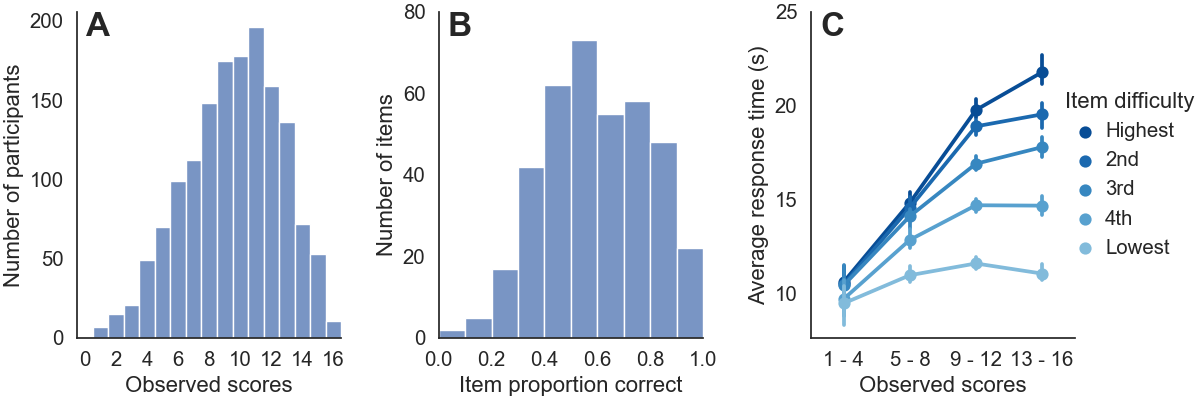
\includegraphics[width=1.0\textwidth]{figures/fig01.png}
\caption{\label{fig:fig01}This is a figure caption.}
\end{figure}
 
\subsection{Item response models}

Reflecting the inherent hierarchical structure of the MaRs-IB -- 80 item families with six clones each -- we estimated the psychometric properties of each item using item cloning models \citep{geerlings2011modeling, cho2014additive, lathrop2017item}. All models were extensions of the three-parameter logistic (3PL) item repsonse model, where the probability of a correct response ($y_{ijk} = 1$) for person $i$ on item clone $k$ belonging to item family $j$ is:

\begin{equation}
p(y_{ijk} = 1) = \gamma_{jk} + (1-\gamma_{jk}) \cdot \text{logit}^{-1} \left( \alpha_{jk} \cdot \theta_i - \beta_{jk} \right)
\end{equation}

\noindent where $\theta_i$ is the latent ability for person $i$, and $\beta_{jk}$, $\alpha_{jk}$, and $\gamma_{jk}$ are the difficulty, discrimination, and guessing parameters for item clone $k$ of item family $j$. Because guessing parameters are difficult to estimate without very large amounts of data \citep{han2012fixing}, we fixed the guessing rate for each item to the nominal rate ($\gamma_{jk} = 0.25$).

To account for the nested structure of the MaRs-IB, the item difficulty and discrimination parameters were estimated using an additive multilevel item structure model \citep{cho2014additive}. Specifically, the difficulty of item clone $k$ belonging to item family $j$ was expressed as:  

\begin{equation}
\beta_{jk} = \mu_\beta + \sum_{n=1}^N Q_{jn} \delta_{\beta n} + \epsilon_{\beta j} + \sum_{m=1}^M R_{km} \delta_{\beta m} + \epsilon_{\beta k}
\end{equation}

\noindent The difficulty parameter is thus modeled as an intercept ($\mu_\beta$), reflecting the average difficulty across all items, and four components:

\begin{enumerate}

\item $\sum_{n=1}^N Q_{jn} \delta_{\beta n}$: the effect of the level-1 attributes, where $Q_{jn}$ is the value of attribute $n$ for item family $j$, and $\delta_{\beta n}$ is the effect of attribute $n$. This component is the fixed effects contribution of item family attributes to item difficulty.

\item $\epsilon_{\beta j}$: the level-1 residual, or variance unexplained by the item family attributes. This component is the random effects contribution of item family attributes to item difficulty.

\item $\sum_{m=1}^M R_{km} \delta_{\beta m}$: the effect of the level-2 attributes, where $R_{km}$ is the value of attribute $m$ for item clone $k$, and $\delta_{\beta m}$ is the effect of attribute $m$. This component is the fixed effects contribution of item clone attributes to item difficulty.

\item $\epsilon_{\beta k}$: the level-2 residual, or variance unexplained by the item clone attributes. This component is the random effects contribution of item clone attributes to item difficulty.

\end{enumerate}

To elaborate, level-1 attributes describe the properties of an item family. Here we model the effects of two properties: feature number, or the number of unique shapes in each cell of an item; and rule number, or the number of changing relationships among the shapes (e.g. color change, shape change, position change) one has to consider in order to correctly solve the item. Example items illustrating these attributes are included in the Supplement.  Note that this definition of item rules deviates from other established taxonomies of matrix reasoning items \citep{carpenter1990one}, a point we return to in the Discussion.

In turn, level-2 attributes describe properties of an item clone. Here we model the effects of two additional properties: distractor type, or whether the distractors were generated following the minimal difference (MD) strategy and a paired difference (PD) strategy (see \cite{chierchia2019matrix} for details); and mean response time, or the average time it took to complete that item. The latter attribute was orthogonalized with respect to the three other item attributes and thus reflects any residual structure after accounting for all other modeled effects. 

Similarly, item discrimination parameters were also expressed as the sum of an equivalent set of components:

\begin{equation}
\alpha_{jk} = \mu_\alpha + \sum_{n=1}^N Q_{jn} \delta_{\alpha n} + \epsilon_{\alpha j} + \sum_{m=1}^M R_{km} \delta_{\alpha m} + \epsilon_{\alpha k}
\end{equation}

\noindent The fixed effect components of the item discrimination parameters were estimated using the same level-1 and level-2 attributes as for the item difficulty parameters (i.e. number of features, number of rules, distractor type, average response time). During estimation, the item discrimination parameters were restricted to be in the range $\alpha_{jk} \in [0, 5]$.

Though complex, the item structure model above provides a natural way of measuring the quality of the MaRs-IB. In the perfect situation, the clones of each item family would be psychometrically equivalent. So too should item families with identical attributes (e.g. number of features, number of rules). This is, of course, unlikely in actuality and the item cloning model allows us to quantify the extent to which equivalent families and clones vary in their difficulty and discrimination. 

To quantify the success of the item cloning process, we estimated a series of four models \citep{cho2014additive, lathrop2017item}: 

\begin{enumerate}

\item \textit{Model 1}: Item parameters are expressed only as a function of their level-1 attributes. This model treats all clones within a family as interchangeable and all item families with the same attributes as equivalent. 

\item \textit{Model 2}: Item parameters are expressed as a function of their level-1 attributes and residuals. This model treats all clones within a family as interchangeable, but now item families with the same attributes may psychometrically vary. 

\item \textit{Model 3}: Item parameters are expressed as a function of their level-1 attributes, level-2 attributes, and level-1 residuals. This model allows clones within a family to vary, but all variation must be explained solely through their attributes.  

\item \textit{Model 4}: Item parameters are expressed as a function of their level-1/2 attributes residuals. The full model in which item families and clones may vary in their psychometric properties. 

\end{enumerate}

The resulting models were then submitted to model comparison. This procedure allows us to measure the success of the item generation process. If the psychometric properties of item families reflect only their attributes, then Model 1 should be preferred to Model 2; in contrast, if item families vary in their properties above and beyond what their attributes can explain, then Model 2 should be preferred. Similarly, if the clones of item family are truly equivalent, then Models 1 or 2 should be preferred to Models 3 or 4; in contrast, if item clones vary substantially (systematically or otherwise), then Models 3 or 4 should be preferred to Models 1 or 2.

Finally, we estimated person-level abilities following an item response modeling approach \citep{wilson2008explanatory}:   

\begin{equation}
\theta_i = \sum_{p=1}^P X_{ip} \rho_p + \epsilon_i    
\end{equation}

\noindent where $X_{ip}$ is the value of attribute $p$ for person $i$, $\rho_p$ is the effect of attribute $n$, and $\epsilon_i$ is variance in ability unexplained by the person-level attributes.

We modeled person-level abilities as a function of four attributes: age, gender (coded as: male = -0.5, female = 0.5; all else = 0), average response time, and $\Delta$ response time. The last term reflected a person's adjustment of their response time as a function of item difficulty (defined as its corresponding proportion of correct responses), and thus measured a participant's tendency to slow down (or speed up) in response to more challenging items.

To ensure the identifiability of all models, person abilities were assumed to be $\theta_i \sim \mathcal{N} \left(0,1\right)$. 

\begin{equation}
blah 
\end{equation}

All models were estimated within a Bayesian framework using Hamiltonian Monte Carlo as implemented in Stan (v2.26) \citep{carpenter2017stan}. For all models, four separate chains with randomised start values each took 7500 samples from the posterior. The first 5000 samples from each chain were discarded. As a result, 10000 post-warmup samples from the joint posterior were retained. The $\hat{R}$ values for all parameters was less than 1.01, indicating acceptable convergence between chains, and there were no divergent transitions in any chain. 

Models were compared using Bayesian leave-one out cross-validation \citep{vehtari2017practical}, which has been found to perform better than other information criteria for comparing item response models \citep{luo2017performances}. Importantly, we computed the marginalized leave-one-cluster out (LOCO) cross-validation \citep{merkle2019bayesian}, which measures models' ability to generalize to held out items (rather than held out responses). 

The fit of the winning model to the data was evaluated through several approaches. First, the fit of the models to the data was assessed by means of posterior predictive model checking \citep{gelman1996posterior}. Item fit was assessed using two two discrepancy statistics: Orlando and Thissen index ($S-\chi^2$) \citep{toribio2011discrepancy} and the generalized dimensionality discrepancy measure (GDDM) \citep{levy2009posterior, levy2011generalized}. The $S-\chi^2$ index is a measure of item fit based on the comparison of observed and expected proportions of participants who answer an item correctly at each raw-score group. The GDDM is a measure to test the model's unidimensionality assumption, which must not be violated in order to compute valid total scores from tests assembled from MaRs-IB items.

\subsection{Model comparison}

First we estimated Models 1-4 holding constant the item discrimination parameters ($\alpha = 1$), which allowed us to investigate the difficulty of MaRs-IB items independently. (Note that these models still included guessing parameters fixed to the nominal guessing rate. We also estimated models with no guessing parameter, i.e. 1PL or Rasch models, but model comparison revealed these to be inferior.) The goodness of fit of the four models was compared based on leave-one-cluster out (LOCO) cross-validation as summarized in Table \ref{table:1}. 

First, Model 2 was preferred to Model 1 suggesting that there is variability in the difficulty of item families above and beyond what can be explained by their attributes. Similarly, Model 3 was preferred to Model 2 suggesting that there is systematic variability in the clones of each item family. Finally, Model 4 was preferred to Model 3 suggesting that there is variability in the difficulty of item clones above and beyond what can be explained by their respective attributes. In summary, the full model -- including all fixed and random effect terms -- was preferred to the three simpler models, indicating that item families and clones are nonequivalent even after controlling for their attributes.

On average, items were difficult (95\% HDI), but ranged considerably in difficulty. Over half of the variability in item difficulty (65.6\%) was explained by the fixed effects of item family (level-1) and clone (level-2) attributes. The associations between level-1 attributes and item difficulty were as expected: feature number was positively associated with difficulty (beta), such that the inclusion of one additional feature was associated with a 13.1\% reduction in expected accuracy. Similarly, rule number was positively associated with item difficulty (beta), such that the inclusion of one additional rule a 10.1\% reduction in expected accuracy. Turning next to level-2 attributes, distractor type was unexpectedly associated with item difficulty (beta), such that clones with MD distractors clones were associated with a 13.6\% reduction in accuracy compared to clones with PD distractors. This pattern is clearly evident in the raw item-level scores (Figure XX). Finally, average response time was positively associated with difficulty, such that a one standard deviation change in response time was associated with an 11.8\% reduction in accuracy. 

The inclusion of item family (level-1) random effects explained an additional 18.5\% of the variance in item difficulty. In total, the percentage of variance in item difficulty not explained by residual variance from item clones (level-2) was 84.1\%. The residual variance was harder to explain (Figure XXb); indeed, there was no clear patterns in difficulty by item set, suggesting that at least part of residual variance may be explained by idiosynchratic perceptual features of item clones. 

Next we estimated three models as above, but with two key differences: First, we no longer held constant the item discrimination parameters but rather estimated them alongside the item difficulty parameters. Second, whereas the item difficulty parameters were always estimated using the full additive multilevel item structure model (i.e. level-1/2 fixed and random effects), the item discrimination parameters were estimated adding one additional component per model (Model 1: level-1/2 fixed effects only; Model 2: fixed effects and level-1 random effects; Model 3: full model). The goodness of fit of the three models was again compared based on leave-one-cluster out (LOCO) cross-validation as summarized in Table \ref{table:2}. 

First, all three models including discrimination parameters were preferred to the best-fitting model with discrimination parameters held constant. Model 2 was preferred to Model 1 suggesting that there is variability in the discrimination of item families not accounted for by their attributes. Importantly, Model 2 was preferred to Model 3 such that there was insufficient variability in discrimination in item clones to necessitate additional parameters. We return to this point in the Discussion.

Returning to variance partitioning, just less than half of the variance in item discrimination (44.9\%) was explained by attributes of the explained by attributes of item families and clones. Interestingly, only the number of item rules was positively associated with item discrimination (HDI); no other attributes were credibly related (HDIs here). 

Finally, we turn to explanatory item response modeling. The largest effects were from the response times. Average response time blah. Delta response time blah. Interestingly, we found a negative correlation between age and ability, such that older participants tended to perform worse on average. Finally, we observed a small but credible association between gender and ability. Though we used the colorblind stimulus set, it is possible there was residual perceptual difficulty for men compared to women. Granted, this effect is small.

This paragraph should be on fit. Should mention: simulation study, posterior predictive check, item fit indices, and unidimensionality measure. You should probably review a couple of other RPM validation papers to make sure our methods are straight (e.g. doi.org/10.1037/a0027830)

\subsection{Discussion}

In discussing the success of the MaRs-IB generation process, some things to point out:

1. A lot of variance in item difficulty and discrimination can be explained by inherent features of the items. This is great!

2. Though there is quite a bit of residual variance at the item family level, this is fine as we only modeled two features. A point we return to in the Discussion.

3. At the clone level, it seems clear that item clones are not equivalent w.r.t. difficulty. For one thing, MD vs. PD big. Should describe level-2 standard deviation somewhere. 

4. For clone discrimination, it seems less clear. One possibility is that there isn't much variability (cite Embertson). Another possibility is that we are underpowered. Cite Lathrop here for discussion of potential bias.

Summarize as good to go!

\section{Test assembly}

With 64 items, each with six clones, there is a vast universe of possible test forms we could construct. Beginning with our motivating problem -- abbreviated measures of nonverbal reasoning with the potential for retest -- we opted to construct three parallel short form measures. To do so, we used mixed integer programming \citep{der2005wj} to maximize the test information function (TIF) of each short form subject to the following constraints:

\begin{enumerate}

    \item Each short form was required to contain 12 items. This was chosen to minimize administration time of a form (2-4 minutes on average) and to achieve sufficient  reliability (Cronbach's $\alpha \geq 0.8$ in piloting).
    
    \item All short forms were required to be comprised of clones from the same item families. This was chosen to maximize the similarity of the short forms.
    
    \item Assigned clones could be of the MD or PD distractor type, but not both. This was chosen to prevent item overlap, as sometimes the MD and PD distractor strategies generate identical distractors.
    
    \item The difference in TIFs across short forms was required to be minimized. This was chosen to ensure that each short form had similar psychometric properties. 
    
\end{enumerate}

\noindent The TIF was maximized at five ability levels ($\theta = -1.0, -0.5, 0.0, 0.5, 1.0$). Previous simulation studies have shown that target values at three to five well-chosen $\theta$s generally suffice \citep{der2005wj}. Solutions to the mixed integer programming problem were found using the \textit{mip} python package (v1.13.0) \citep{santos2020mixed}.

The test information functions (TIFs) and test characteristic curves (TCCs) for the three short forms are shown in Figure XX. As can be readily observed, the TIFs for each short form are remarkably similar reflecting the constraints of the MIP problem. Thus, the short forms should have similar levels of precision across ability levels. Similarly, the TCCs for each short form are similar, which was by no means guaranteed \citep{ali2016evaluation}. Thus, the short forms are expected to have similar total score distributions.

Thus we proceeded to test each short form. blah blah blah.

\section{Validation Study}

\subsection{Data Collection}

A total of N=347 participants were recruited from the Prolific Academic platform (https://www.prolific.co) to participate in an online behavioral experiment in November, 2021. Participants were eligible if they currently resided in the United States and had not participated in the calibration study. This study was approved by the Institutional Review Board of Princeton University (\#7392), and all participants provided informed consent. Total study duration was approximately 10.8 minutes (4.6 sd) per participant. Participants received monetary compensation for their time (rate USD \$10/hr), plus an incentive-compatible bonus up to \$0.75 based on task performance (average payment: mean = \$2.10 [\$0.18 sd]). 

After providing consent, participants completed the experiment which was divided into three section. In the first, participants completed three short surveys: the 10-item need for cognition survey \citep{chiesi2018applying}, the 8-item PROMIS Cognitive Function-Short Forms (8a) \citep{iverson2021normative}, and the 8-item subject numeracy scale \citep{fagerlin2007measuring}. These measures were included as part of exploratory analyses that were not the central focus of this study and will not be reported in the main text (reported in Supplement). Next, participants completed one of the three 12-item MaRs-IRB short-forms described above. Besides for the items, the administration procedure of the short-forms was identical to that in the Calibration study. Finally, participants completed the 9-item abbreviated Raven's progressive matrices (form A) \citep{bilker2012development}. For consistency's sake, the administration procedure was matched to the MaRs-IB. 

The data from a total of N=47 participants were excluded prior to analysis. Of these, N=17 participants were excluded for having not completed the entire experiment. Separately, the data from N=21 participants were excluded for failing one or more attention checks (infrequency items) embedded in the self-report measures \citep{zorowitz2021inattentive}. The data from N=13 participants were excluded for image loading problems on either the MaRs-IB or RPM tasks. Finally, N=6 participants were excluded for missing or rapid guessing on 4 or more trials during the MaRs-IB or RPM tasks. Note these are not mutually exclusive.

The majority of participants in the validation sample identified as women (men: N=138; women: N=147; non-binary or other: N=13; rather not say: N=2). Participants were 35.0 years old (13.2 sd) on average. The sample was relatively well-educated with the majority having a Bachelor's degree (N=121) or Master's degree or higher (N=45); fewer participants endorsed only completing some college (N=100) or only a high school degree or lower (N=33). 

\subsection{Results}

The distribution of scores on the three MaRs-IB short-forms are summarized in Table \ref{table:2}. Across the short-forms, participants responded correctly on 8.0 of 12 items (sd = 2.5, IQR = 6 - 10). The distribution of scores were skewed towards to higher end, as would be expected given their respective test characteristic curves. A 1-way ANOVA did not reject the null hypothesis that the observed scores across test forms were equal (F(2,97) = 0.253, p = 0.777). Corroborating the predictions from the test assembly, the reliability of each short form was satisfactory (Table \ref{table:2}). 

The distribution of scores on the RPM short-form is similarly summarized in Table \ref{table:2}. On average, participants responded correctly on 4.5 of 9 items (sd = 2.0, IQR = 3 - 9). Scores on the RPM were significantly lower on the RPM than the MaRs-IB ($t = 25.598, p < 1e^{-6}$), indicating that the items on the RPM short-form are more difficult on average than those selected for the MaRs-IB short-forms. The reliability of the measure was similarly good as the MaRs-IB (Table \ref{table:2}). 

To measure convergent validity, blah blah blah. Need to write model here. Or should we write above?

\subsection{Discussion}

\section{General Discussion}

Paragraph XX: item discrimination random effects. Power analysis? also variance explained being similar to literature.

-----
Notes on RT effects: this paragraph should come later, as a discussion point on what we're actually measuring with the MaRs-IB (at least online)

Heitz (2014): in general, an increase in speed comes at the expense of accuracy (speed-accuracy trade-off)

Goldhammer (2015): 

> Individual differences in test performance depend on both between-person differences in speed and ability (i.e., the location of individual speed-ability curves) and the adopted speed-ability compromise within persons (i.e., the location within a speed-ability curve). T

Goldhammer et al. (2015): test takers that increase their work pace have a lower effective ability

> On previous reasoning tasks: "These findings indicate that in tasks that require understanding new problem situations and in which the use of complex cognitive processes is mandatory, higher effective ability is usually associated with lower speed." 

Ranger et al. (2021): 

> Such a relation between response time and response accuracy or between work pace and effective ability is of uttermost importance as it implies that the responses depend on more than just the test taker’s capability.

> the capability is apportioned among two quantities, the effective ability, and the work pace, which constitute the actual performance of a test taker in a test; see Pohl and von Davier (2018) for a discussion on how to describe the performance of test takers. 

As work pace increases, effective ability decreases (irrespective of true capability). Work rate may reflect other processes: persistence, or amount of time before participant gives up, mental effort costs, or foraging costs.  

Basically, summarize results. All points are consistent with dual process theory (automatic vs. controlled processing). suggestins higher ability participants more deliberate, lower ability participants less deliberate. frame from perspective of persistence (ranger 2021).

Need to cite: https://doi.org/10.1016/j.intell.2020.101490

-----

Paragraph XX: future directions modeling speed-accuracy trade-offs

Paragraph XX: model more features as future direction. Carpenter taxonomy. Model by rule type. By perceptual features. automatic item generation as future direction. See \cite{lathrop2017item} for inspiration.

\bibliography{example}

\begin{table}
\centering
\begin{tabular}{l|c|c|c}
Model & elpd$_{loco}$ & loco & $\Delta$ loco \\\hline
1PG-F &  & -14516 & \\
1PG-FX &  & -13804 & \\
1PG-R &  & -13481 & \\
1PG-RX &  & -13293 & - \\
\end{tabular}
\caption{Table to test captions and labels.}
\label{table:1}
\end{table}

\begin{table}
    \centering
    \begin{tabular}{c|c|c|c}
    Measure & Mean (sd) & IQR & Reliability \\
    \hline
    MaRs-IB SFa & 7.9 (2.4) & 7 - 10 & 0.761 \\
    MaRs-IB SFb & 8.2 (2.6) & 7 - 10 & 0.810 \\
    MaRs-IB SFc & 7.9 (2.7) & 6 - 10 & 0.829 \\
    RPM SFa & 4.5 (2.0) & 3 - 9 & 0.791 \\
    \end{tabular}
    \caption{Caption}
    \label{table:2}
\end{table}

\end{document}
